\documentclass{article}

\usepackage{tikz}

\begin{document}
	\begin{figure}[h!]
	\begin{center}
		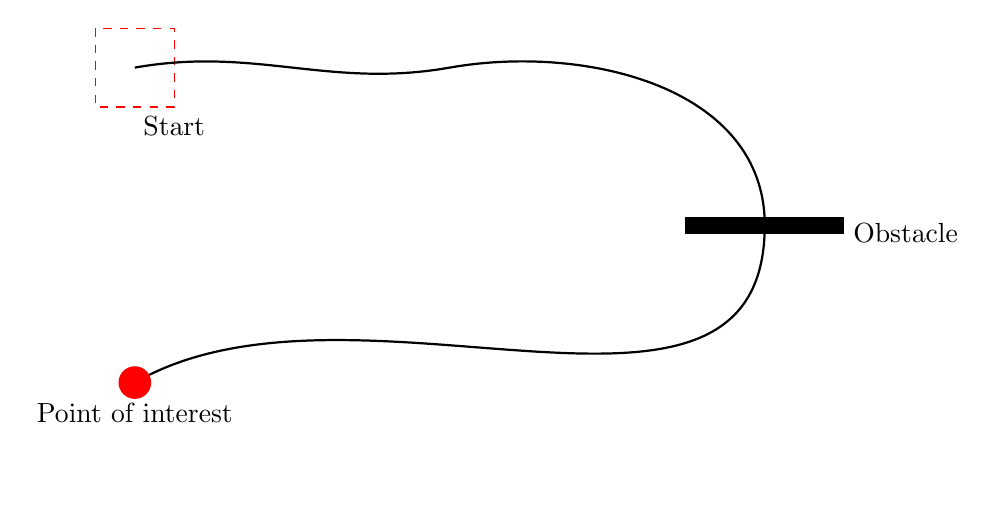
\begin{tikzpicture}
			% draws a rectangle
			\draw [red,dashed] (-2.5,2.5) rectangle (-1.5,1.5) node [black,below] {Start};
			\draw [thick] (-2,2) % Draws a line
				to [out=10,in=190] (2,2)
				to [out=10,in=90] (6,0) 
				to [out=-90,in=30] (-2,-2);    
			% draws another rectangle
			\draw [fill] (5,0.1) rectangle (7,-0.1) node [black,right] {Obstacle};
			% draws a circle
			\draw [red,fill] (-2,-2) circle [radius=0.2] node [black,below=4] {Point of interest};
		\end{tikzpicture}
		\caption{Example graphic made with tikz.}
	\end{center}
	\end{figure}
\end{document}
